\documentclass[tikz]{standalone}
\usepackage{tikz}

\begin{document}    
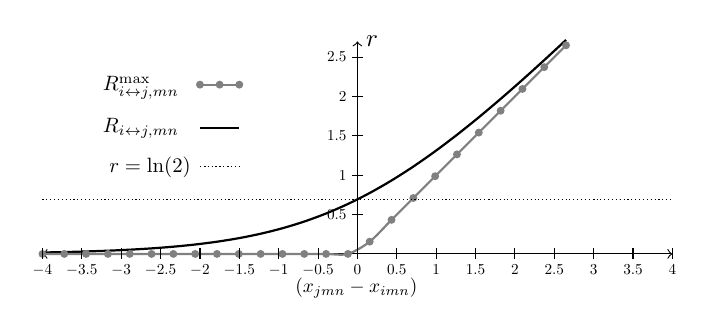
\begin{tikzpicture}
 \usetikzlibrary{positioning}
 \node (center) {};
 
 
 %Coordinates
 \coordinate (maxRRMcoordinate) at (1.1,0.9);
 \coordinate (RRMcoordinate) at (0.5,1);
 \coordinate (ln2coordinate) at (-2.5,{ln(2)});
 
 
 %Names
 \node (maxRRM) [scale=0.75,above left=1.75cm and 2.05cm of center  ] {$R^{\max}_{i\leftrightarrow j,mn}$};
   \draw[scale=1, domain=-2:-1.5, gray ,thick,mark=*,samples=3,mark options={scale=0.5} ] plot  ({\x}, {2.15});
 
 \node (RRM) [scale=0.75, above left=1.25cm and 2.05cm of center] { $R_{i\leftrightarrow j,mn}$};
   \draw[scale=1, domain=-2:-1.5, smooth ,variable=\x, black,thick  ] plot  ({\x}, {1.6}); 
 
 \node (ln2name) [scale=0.75, above left=0.75cm and 1.9cm of center] { $r=\ln(2)$};
    \draw[scale=1, domain=-2:-1.5, densely dotted, variable=\x, black ] plot  ({\x}, {1.11});
 
 %Axis
   \draw[<->] (-4, 0) -- (4, 0) node[scale=0.7, below right = 0.1cm and -1cm of center] {$(x_{jmn} - x_{imn})$};
  \draw[->] (0, 0) -- (0, 2.7) node[right,scale=0.9] {$r$};
  
 %Functions 
  \draw[scale=1, domain=-4:2.65, smooth ,variable=\x, black,thick  ] plot  ({\x}, {ln(1+exp(\x))});
  \draw[scale=1, domain=-4:2.65, smooth, variable=\x, gray ,thick,mark=*,mark options={scale=0.5}] plot ({\x}, {max(0,\x)});

  \draw[scale=1, domain=-4:4, densely dotted, variable=\x, black] plot ({\x}, {ln(2)});

 \foreach \x/\xtext in {0,0.5,1,1.5,2,2.5,3,3.5,4}
\draw[shift={(\x,0)}] (0pt,2pt) -- (0pt,-2pt) node[scale=0.55,below] {$\xtext$};

 \foreach \x/\xtext in {0.5,1,1.5,2,2.5,3,3.5,4}
\draw[shift={(-\x,0)}] (0pt,2pt) -- (0pt,-2pt) node[scale=0.55,below] {$-\xtext$};

  \foreach \y/\ytext in {0.5,1,1.5,2,2.5}
  \draw[shift={(0,\y)}] (2pt,0pt) -- (-2pt,0pt) node[scale=0.55,left] {$\ytext$};
  %Labels of functions

 % \draw[->] (maxRRM) -- (maxRRMcoordinate);
 % \draw[->] (RRM) -- (RRMcoordinate);
 %  \draw[->] (ln2name) -- (ln2coordinate);
  
\end{tikzpicture}
\end{document}


